%\Large\mathphyssubsubsec{Lehramt Informatik}\normalfont\small
\section{50\%-Bachelor Informatik (Lehramt)}
\sidebar{
	\centering
	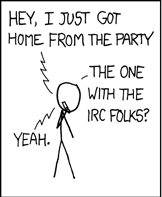
\includegraphics[width=3.5cm]{bilder/xkcd_responsible_behaviour_1.png}\\\vspace{10mm}
	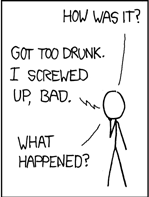
\includegraphics[width=3.5cm]{bilder/xkcd_responsible_behaviour_2.png}\\\vspace{10mm}
	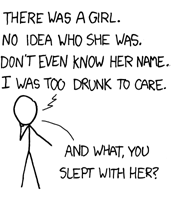
\includegraphics[width=3.5cm]{bilder/xkcd_responsible_behaviour_3.png}\\\vspace{10mm}
	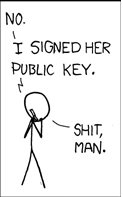
\includegraphics[width=3.1cm]{bilder/xkcd_responsible_behaviour_4.png}
}

Wenn ihr den 50\%-Bachelor Informatik studiert, sind zwei Fälle zu
unterscheiden: Entweder hört ihr in eurem zweiten Fach
Mathematik-Veranstaltungen oder ihr tut es nicht. Diese Unterscheidung rührt
daher, dass ihr in der Informatik auf jeden Fall etwas Mathematik können
solltet. Wenn ihr in eurem anderen Fach Mathe hört, habt ihr das aber schon da
abgedeckt und könnt euch in dieser Hälfte eures Bachelors ganz auf die
Informatik konzentrieren.

Auf jeden Fall hört ihr im ersten Semester \hyperref[info1]{„Einführung in die
Praktische Informatik“ (Info 1)} und den Programmierkurs. Hier ist besonders
die erste Veranstaltung wichtig, da es euere Orientierungsprüfung in Informatik
ist. Im zweiten Semester solltet ihr dann in Informatik die „Einführung in die
Theoretische Informatik“ \footnote{„Theo“ kann zu Verwirungen mit Physikern
führen, da diese das als „Theoretische Physik“ verstehen} und „Algorithmen und
Datenstrukturen“ (AlDa) hören. Im Dritten Semester macht sich der Unterschied,
ob ihr in eurem zweiten Fach Mathe hört, bemerkbar, da ihr hier
„Mathematik für Informatiker 1“ (MafIn 1)  hören sollt.  Wenn ihr aber bereits
andere Matheveranstaltungen bestanden habt, könnt ihr beim Prüfungsausschuss
beantragen, dass ihr stattdessen ein weiteres Info-Modul aus den
Wahlpflicht-Veranstaltungen hören könnt.  Ausserdem ist vorgesehen das ihr im
Dritten Semester die „Einführung in die Technische Informatik“ (ITE oder
Technische Info)\footnote{dafür hat leider noch niemand eine schön Abkürzung
gefunden} hört.  Im Vierten und Fünften Semester stehen dann „Betriebssysteme
und Netzwerke“ (BeNe), „Software Engineering“ (ISW) und ein Proseminar auf dem
Plan. Im sechsten Semester müsst ihr dann neben der Bachelorarbeit, die ihr in
einem eurer beiden Fächer schreibt, noch „Datenbanken 1“ (IDB1) hören. Hinzu
kommen dann noch ein Anfängerparktikum und ein Seminar. Falls ihr nach dem
Bachelor den „Master of Education“ machen wollt, müsst ihr das Proseminar und
das Anfängerpraktikum im Themenbereich „Informatik und Gesellschaft“ (IuG)
machen.  Da im Seminar und Proseminar und Seminar schon LP als
„Fachübergreifende Kompetenzen“ (FÜK) vergeben werden habt ihr nun noch 4 LP
die ihr mit einer FÜK Veranstaltung eurer Wahl holen könnt.

Ihr solltet euch bei jeder Veranstaltung genau darüber informieren, was ihr
benötigt, um zur Prüfung zugelassen zu werden (z.B. 50\% auf den Übungszetteln)
und was genau \emph{eine} Prüfung beinhaltet (z.\,B.\ das Bestehen von einer von
zwei Klausuren). Insbesondere der letzte Teil ist wichtig, denn ihr könnt
Prüfungen grundsätzlich zweimal versuchen. Je nach Veranstaltung und Dozent/in
\emph{können} zwei Klausuren als eine Prüfung zählen, müssen aber nicht -- dann
würde jede geschriebene Klausur als ein Prüfungsversuch gelten. Wenn ihr aus
Gründen, die ihr nicht zu verantworten habt (wie krank sein), nicht an einer
\emph{Prüfung} teilnehmen konntet, erhöhen sich entsprechend eure Versuche.
Wenn ihr alle \emph{Klausur}termine verpasst habt, kann die Klausur auch durch
eine mündliche Prüfung ersetzt werden. Sollte das bei euch mal der Fall sein,
fragt ihr jedoch am besten den/die Dozent/in.

Im 50\%-Bachelor habt ihr leider nur sehr wenig Wahlmöglichkeiten, da die
meisten Veranstaltungen verpflichtend sind.  Einen Anhaltspunkt für die Planung
eures Studiums können die Musterstudienpläne in eurer Prüfungsordnung sein, die
„nach Vorgabe“ erstellt wurden. Das heißt, sie enthalten ca.\ 15
Leistungspunkte pro Semester und versuchen gleichzeitig, die Veranstaltungen
möglichst sinnvoll anzuordnen.
